\documentclass[a4paper,12pt]{article}

\usepackage[spanish]{babel}
\usepackage[utf8]{inputenc}
\usepackage[T1]{fontenc}
\usepackage[utf8]{inputenc}
\usepackage{makeidx}
\usepackage{graphicx}
\usepackage{lmodern}
\usepackage{kpfonts}
\usepackage[left=2cm,right=2cm,top=2cm,bottom=2cm]{geometry}
\usepackage{amsmath,amsfonts,amssymb}

\title{TAREA 3}
\author{Junior Miguel Lara Torres}
\date{today}

\graphicspath {{C:/Users/JuniorLara/Desktop/TexMaker_Files/}}
\begin{document}

\begin{center}
\par 
\includegraphics[scale=1]{USB} \par
Universidad Simon Bolivar \\ Curso: CI2511 / Logica Simbolica \\ Trimestre: Abril-Julio, 2021 \\ Profesor: Carolina Chang Tovar \\ Estudiante: Junior Miguel Lara Torres - Carnè: 17-10303 \\
\end{center}

\begin{center}
TAREA 3
\end{center}

Dada la expresión: \\

$ \neg p \equiv \neg q \vee (q \equiv \neg q \wedge p \equiv p) \equiv \neg q \wedge (p \equiv q)\equiv \neg q \\ $ \par

- Si la expresión no es un teorema, muestre detalladamente un estado en el que la expresión se evalúe falsa.\par
- Si la expresión es un teorema, demuéstrelo formalmente partiendo de \par
$\\ ~~~~~~~~~~ \neg p \equiv \neg q \vee (q \equiv \neg q \wedge p \equiv p)\\ $ \par

- e indicando X, Y, E en cada paso de la demostración. Se pueden realizar asociatividades, simetrías y doble negación de manera implícita. \\ \par

Solucion: Verificamos por tabla de la verdad, para la expresiòn 

\begin{center}
$E: \neg p \equiv \neg q \vee (q \equiv \neg q \wedge p \equiv p) \equiv \neg q \wedge (p \equiv q)\equiv \neg q$
\end{center} 

\par 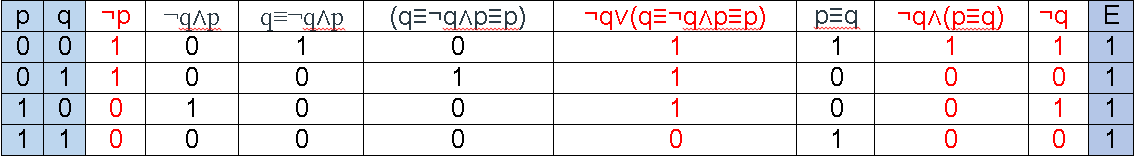
\includegraphics[scale=0.6]{Tabla} \par

Por lo tanto, se demuestrado que para todo estado de la expresiòn E siempre es $True$. Por otra parte, procedemos a demostrar partiendo de \par
$\\                 ~~~~~~~~$ \textbf{$\neg p \equiv \neg q \vee (q \equiv \neg q \wedge p \equiv p)$} $\\ \\ $ 
$\equiv ~~~~~~~~~~ \left\langle~~ \begin{matrix} 
(3.35)~~ (p\wedge q \equiv p \equiv q \equiv p \vee q)[p,q:=\neg q,~p] \\ 
X=\neg q \wedge p
~~Y=\neg q \equiv p \equiv \neg q \vee p,
~~E=\neg p \equiv \neg q \vee (q \equiv z \equiv p)
\end{matrix} ~~\right\rangle \\ \\
                 ~~~~~~~~\neg p \equiv \neg q \vee (q \equiv \neg q \equiv p \equiv \neg q \vee p \equiv p) \\ \\
\equiv ~~~~~~~~~~ \left\langle~~ \begin{matrix} 
(3.27)~~ (p \vee (q \equiv r) \equiv p \vee q \equiv p \vee r)[p,q,r:=\neg q,~p\equiv q,~\neg q \equiv p \equiv \neg q \vee p],~~ \langle \text{Simetrìa de la } \equiv \rangle~, \\ 
X=\neg q \vee (p \equiv q \equiv \neg q \equiv p \equiv \neg q \vee p),
~~Y=\neg q \vee (p \equiv q) \equiv \neg q \vee (\neg q \equiv p \equiv \neg q \vee p),
~~E=\neg p \equiv z
\end{matrix} ~~\right\rangle \\ \\
                 ~~~~~~~~\neg p \equiv \neg q \vee (p \equiv q) \equiv \neg q \vee (\neg q \equiv p \equiv \neg q \vee p)\\ \\
\equiv ~~~~~~~~~~ \left\langle~~ \begin{matrix} 
(3.27)~~ (p \vee (q \equiv r) \equiv p \vee q \equiv p \vee r)[p,q,r:=\neg q,~\neg q,~ p \equiv \neg q \vee p], \\ 
X=\neg q \vee (\neg q \equiv p \equiv \neg q \vee p),
~~Y=\neg q \vee \neg q \equiv \neg q \vee (p \equiv \neg q \vee p),
~~E=\neg p \equiv \neg q \vee (p \equiv q) \equiv z 
\end{matrix} ~~\right\rangle \\ \\
                 ~~~~~~~~\neg p \equiv \neg q \vee (p \equiv q) \equiv \neg q \vee \neg q \equiv \neg q \vee (p \equiv \neg q \vee p)\\ \\
\equiv ~~~~~~~~~~ \left\langle~~ \begin{matrix} 
(3.26)~~ (p \vee p \equiv p)[p:=\neg q], \\ 
X=\neg q \vee \neg q,
~~Y=\neg q,
~~E=\neg p \equiv \neg q \vee (p \equiv q) \equiv z \equiv \neg q \vee (p \equiv \neg q \vee p)
\end{matrix} ~~\right\rangle \\ \\
                 ~~~~~~~~\neg p \equiv \neg q \vee (p \equiv q) \equiv \neg q \equiv \neg q \vee (p \equiv \neg q \vee p)\\ \\
\equiv ~~~~~~~~~~ \left\langle~~ \begin{matrix} 
(3.27)~~ (p \vee (q \equiv r) \equiv p \vee q \equiv p \vee r)[p,q,r:=\neg q,~p,~\neg q \vee p], \\ 
X=\neg q \vee (p \equiv \neg q \vee p),
~~Y=\neg q \vee p \equiv \neg q \vee (\neg q \vee p),
~~E=\neg p \equiv \neg q \vee (p \equiv q) \equiv \neg q \equiv z
\end{matrix} ~~\right\rangle \\ \\
                 ~~~~~~~~\neg p \equiv \neg q \vee (p \equiv q) \equiv \neg q \equiv \neg q \vee p \equiv \neg q \vee (\neg q \vee p)\\ \\
\equiv ~~~~~~~~~~ \left\langle~~ \begin{matrix} 
(3.26)~~ (p \vee p \equiv p)[p:=\neg q],~~ \langle \text{Asociatividad de la }\vee \rangle~, \\
X=\neg q \vee \neg q,
~~Y=\neg q,
~~E=\neg p \equiv \neg q \vee (p \equiv q) \equiv \neg q  \equiv \neg q \vee p \equiv z \vee p
\end{matrix} ~~\right\rangle \\ \\
                 ~~~~~~~~\neg p \equiv \neg q \vee (p \equiv q) \equiv \neg q \equiv \neg q \vee p \equiv \neg q \vee p\\ \\
\equiv ~~~~~~~~~~ \left\langle~~ \begin{matrix} 
~~ (p \equiv p \equiv q \equiv q)[p,q:=\neg q \vee p,~\neg q], \\
X=\neg q \vee p \equiv \neg q \vee p,
~~Y=\neg q \equiv \neg q,
~~E=\neg p \equiv \neg q \vee (p \equiv q) \equiv \neg q \equiv z
\end{matrix} ~~\right\rangle \\ \\
                 ~~~~~~~~\neg p \equiv \neg q \vee (p \equiv q) \equiv \neg q \equiv \neg q \equiv \neg q \\ \\
\equiv ~~~~~~~~~~ \left\langle~~ \begin{matrix} 
(3.11)~~ (\neg p \equiv \neg q \equiv p \equiv q)[p,:=q,~p] ~,~~ \langle \text{Simetrìa de la } \equiv \rangle~, \\
X=\neg q \equiv \neg p,
~~Y=q \equiv p,
~~E= \neg q \equiv z \equiv \neg q \vee (p \equiv q) \equiv \neg q
\end{matrix} ~~\right\rangle \\ \\
                 ~~~~~~~~\neg q \equiv q \equiv p \equiv \neg q \vee (p \equiv q) \equiv \neg q \\ \\
\equiv ~~~~~~~~~~ \left\langle~~ \begin{matrix} 
(3.35)~~ (p\wedge q \equiv p \equiv q \equiv p \vee q)[p,q:=\neg q,~p \equiv q] ~,~~ \langle \text{Simetrìa de la } \equiv \rangle~, \\ 
X=\neg q \equiv p \equiv q \equiv \neg q \vee (p \equiv q),
~~Y=\neg q \wedge (p \equiv q),
~~E= z \equiv \neg q
\end{matrix} ~~\right\rangle \\ \\
                 ~~~~~~~~$ \textbf{$\neg q \wedge (p \equiv q) \equiv \neg q$}$ \\ \\ $ 
                 
Finalmente, debido a la transitividad, hemos probado que;
\begin{center}
$\neg p \equiv \neg q \vee (q \equiv \neg q \wedge p \equiv p) \equiv \neg q \wedge (p \equiv q)\equiv \neg q$
\end{center}

\end{document}
